\section{OD Construction} \label{od_construction_sec}
\par
Design changes and time on side... only a page or 2


\par
This geometry now implemented is still not complete, for example the PMT conduits on top of the OCV do not extend to the edge of the water tank. 

\begin{figure}[!htbp]
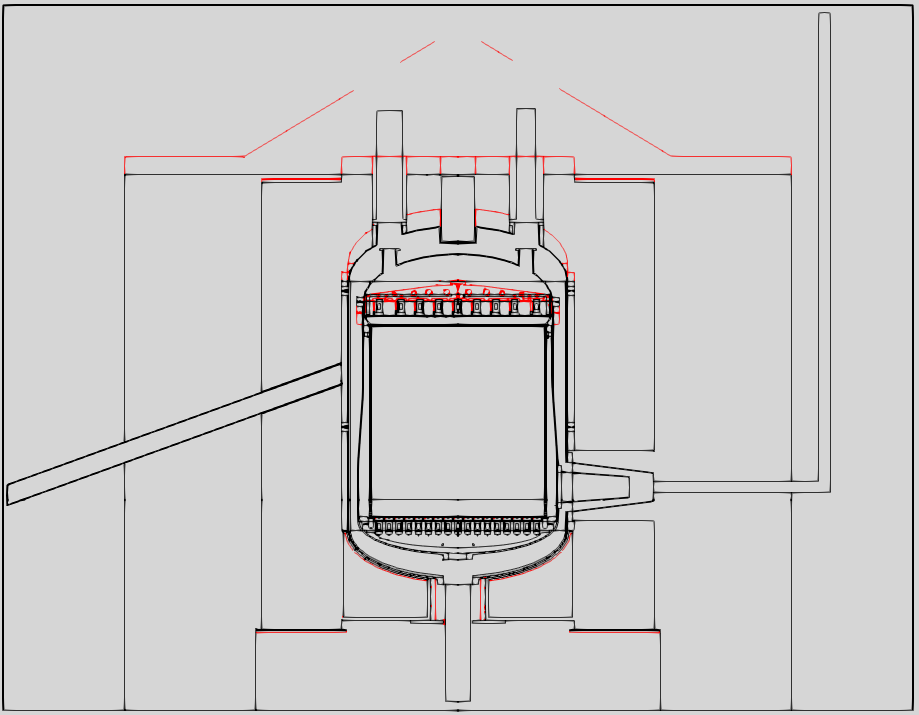
\includegraphics[width=\textwidth]{Figures/Construction/geometry_differences.png}
\centering
\caption{LZ geometry slice as implemented in Geant4 from the water tank in. In black: the designed geometry as in Figure \ref{fig:LZ_Cut_CAD}. In Red: changes to the design including raised Top OD tanks and additional foam. OD PMTs are not shown here due to none lying on this plane.}
\label{fig:Geometry_Differences}
\end{figure}


\begin{table}[!htbp]
    \centering
    \begin{tabular}{ c | c | c } 
    \hline
    \multirow{2}{*}{Volume} & \multicolumn{2}{l}{Percentage captured in volume (\%)} \\ 
                            & All Neutrons  & SS and FID  \\ \hline
    volA    & 0.0   & 1232\\
    volB    & 0.0   &
    \end{tabular}
    \caption{Fraction of background neutrons captured in various detector volumes}
    \label{tab:fraction_of_neutrons_captured_in_volumes}
\end{table} 